\documentclass{article}
\usepackage{graphicx}
\usepackage[utf8]{inputenc}
\usepackage[T1]{fontenc}
\usepackage{fouriernc}
\usepackage[margin=1in]{geometry}
\usepackage{amsmath}
\usepackage{wrapfig}
\usepackage{fancyhdr}
\usepackage{listings}
\usepackage{xcolor}
\usepackage{caption}
\usepackage{hyperref}
\hypersetup{
    colorlinks=true,
    linkcolor=black,
    urlcolor=blue,
}

\urlstyle{same}
\usepackage{subcaption}
\definecolor{codegreen}{rgb}{0,0.6,0}
\definecolor{codegray}{rgb}{0.5,0.5,0.5}
\definecolor{codepurple}{rgb}{0.58,0,0.82}
\definecolor{backcolour}{rgb}{0.95,0.95,0.92}

\lstdefinestyle{mystyle}{
    backgroundcolor=\color{backcolour},   
    commentstyle=\color{codegreen},
    keywordstyle=\color{magenta},
    numberstyle=\tiny\color{codegray},
    stringstyle=\color{codepurple},
    basicstyle=\ttfamily\footnotesize,
    breakatwhitespace=false,         
    breaklines=true,                 
    captionpos=b,                    
    keepspaces=true,                 
    numbers=left,                    
    numbersep=5pt,                  
    showspaces=false,                
    showstringspaces=false,
    showtabs=false,                  
    tabsize=2
}

\lstset{style=mystyle}
\pagestyle{fancy}
\fancyhf{}
\rhead{201701073 | 201701074}
\lhead{HPC - Floyd-Warshall Parallelization}
\rfoot{\thepage}
\begin{document}

\begin{titlepage}
	\centering 
	\scshape
	\vspace*{12\baselineskip}
	\rule{\textwidth}{1.6pt}\vspace*{-\baselineskip}\vspace*{2pt}
	\rule{\textwidth}{0.4pt} 
	\vspace{0.75\baselineskip}
	
	{\Large CS 301 : High Performance Computing \\\vspace{0.75\baselineskip} Floyd-Warshall Parallelization}
	\vspace{0.75\baselineskip}
	
	\rule{\textwidth}{0.4pt}\vspace*{-\baselineskip}\vspace{3.2pt} 
	\rule{\textwidth}{1.6pt}
	
	
	\vspace*{3\baselineskip}
	{\scshape\large Assigned By\\ Prof. Bhaskar Chaudhury}
	
	\vspace{3\baselineskip} %originally 0.5
	
	
	{\scshape\large Students\\Purvil Mehta (201701073) \\ Bhargey Mehta (201701074) \\} 
	
	\vspace{1\baselineskip} 
	
	\textit{Dhirubhai Ambani Institute of Information and Communication Technology \\ Gandhinagar\\} 
	\vspace*{2\baselineskip}
	\today


\end{titlepage}
\newpage
\tableofcontents



% \section{Serial Implementation}

% \begin{lstlisting}[language=C ,caption=Serial Code]
% for(k=0; k<N; k++){
% 	for(i=0; i<N; i++){
% 		for(j=0; j<N; j++){
% 			if(dis[i][j] > dis[i][k]+dis[k][j])
% 				dis[i][j] = dis[i][k]+dis[k][j];
% 		}
% 	}
% }
% \end{lstlisting}

% \subsection{Memory Access Strategy in Serial Code}
% \begin{itemize}
%     \item Since this algorithm contains initial 2D matrix which shows the distance between any two node, We run our code in two ways. 
%     \begin{enumerate}
%         \item \textbf{2D Memory Allocation using malloc :} Since the value inside the matrix will be flatten in the real memory system,this approach takes longer time to run because of its two reference pointer i and j which guide them to the proper memory location.
%         \begin{lstlisting}[language=C, caption=2D Memory Allocation using malloc]
% int **adj_mat = (int*)malloc(N*sizeof(int));
% int **dis = (int*)malloc(N*sizeof(int));
% for(i=0; i<N;++i){
%     adj_mat[i] = (int*)malloc(N*sizeof(int));
%     dist[i] = (int*)malloc(N*sizeof(int));
% }
% \end{lstlisting}
%         \item \textbf{Continuous Memory Allocation:} In this case we flatten the whole 2D array into 1D array. So whenever there is a need of any element in the matrix, the reference pointer only need to search for the location of j and directly jump to the location pointed by i. 
%         \begin{lstlisting}[language=C, caption=Continuous Memory Allocation]
% int (*adj_mat)[N] = malloc(N * sizeof(*adj_mat));
% int (*dis)[N] = malloc(N * sizeof(*adj_mat));
% \end{lstlisting}
%     \end{enumerate}
    
%     \item Since the memory access time and cache miss rate are lesser in the second approach, we found that the serial code with strategy second was taking \textbf{205 seconds} on and average. Whereas, the serial code with strategy first was taking \textbf{225 seconds} on and average
% \end{itemize}

% \newpage

\newpage
%%%%%%%%%%%%%%%%%%%%%%%%%%%%%%%%%%%%%%%%%%%%%%%%%%%%%%%%%%%%
%%%%%%%%%%%%%%%%%%%%%%%%%%%%%%%%%%%%%%%%%%%%%%%%%%%%%%%%%%%%%
%%%%%%%%%%%%%%%%%%%%%%%%%%%%%%%%%%%%%%%%%%%%%%%%%%%%%%%%%%%%5
%%%%%%%%%%%%%%%%%%%%%%%%%%%%%%%%%%%%%%%%%%%%%%%%%%%%%%%%%%%%%

\section{Brief Introduction}
The Floyd–Warshall algorithm (also known as Floyd's algorithm, the Roy–Warshall algorithm, the Roy–Floyd algorithm, or the WFI algorithm) is an algorithm for finding shortest paths in a weighted graph with positive or negative edge weights (but with no negative cycles). This algorithm will find the shortest distance possible to any of the two nodes. We will later prove that maximum achievable speedup is $p$. Our aim is to optimize the cache usage in such a way that we achieve a speedup as close as possible to this upper bound.

\subsection{Input}
The input contains a graph of $N$ nodes and their edge weights in the form of an adjacency matrix of size $N \times N$. This algorithm can handle negative edge weights but not negative cycles since if there does exist a negative cycle then we can circle to this cycle, go around it an infinite number of times and have a distance of $- \infty$ between all nodes. There doesn't remain a need of the algorithm in the first place.

More formally \texttt{adj\_mat[i][j]} denotes the weight of the edge that originates in node i and terminates in node j. In case of an un-directed graph, \texttt{adj\_mat[i][j]} =  \texttt{adj\_mat[j][i]}.


\subsection{Output}
The output is a matrix \texttt{dis} of size $N \times N$. This means that the optimum distance for going from node i to j is the value \texttt{dis[i][j]}. Again in case of an undirected graph, we will get \texttt{dis[i][j]} =  \texttt{dis[j][i]}. 

\section{Algorithm}
The algorithm works by considering a set of nodes which act as intermediate nodes between a given source and sink. This means that for a given source and sink, we have the optimum distance when the intermediate nodes are allowed to be from this set. 


With each iteration of the algorithm, we expand this set. According to the definition of the $\mathrm{k}^{\mathrm{th}}$ iteration, we should obtain the optimum distance when the intermediate nodes allowed to be from the set ${1, 2, .., k}$. The node $k$ is now allowed to be an intermediate node so some paths, let's say from $i$ to $j$ would be updated but one condition that holds true is that $d(i, k)$ and $d(k, j)$ won't change in this iteration or that they are already optimum. This holds true because we are disallowing negative cycles.

\begin{itemize}
    \item We initialize the solution matrix same as the input graph matrix as a first step. That is to say that there are no intermediate nodes. All the edges themselves are the optimum distance.
    \item Each iteration is the inclusion of the node $k$. For every pair $(i, j)$ of the source and destination nodes respectively, there are two possible cases.
    \begin{enumerate}
        \item k is not an intermediate node in shortest path from i to j. We keep the value of \textbf{dist[i][j]} as it is.
        \item k is an intermediate node in shortest path from i to j. We update the value of \textbf{dist[i][j]} as \textbf{dist[i][k] + dist[k][j] if dist[i][j] > dist[i][k] + dist[k][j].}
    \end{enumerate}
\end{itemize}

\section{Scope of Parallelism}
We will prove that \texttt{dis[i][k]} will not be updated during the $\mathrm{k}^{\mathrm{th}}$ iteration. For that statement to be executed,
$$\texttt{dis[i][k]} > \texttt{dis[i][k]}+\texttt{dis[k][k]}$$
$$\texttt{dis[k][k]} < 0$$
This can't be true since this implies a negative cycle and we have forbidden that. We can similarly prove that \texttt{dis[k][j]} will also not be updated. \\ \\
Hence \texttt{dis[i][j]} always depends on two quantities which are not going to be updated. Hence there will be no data race, only parallel reads. Hence the one singular iteration of $N^2$ updates can safely be parallelised.

\subsection{Serial Fraction of the code}
\begin{enumerate}
    \item The statement \texttt{dis[i][j]} = min(\texttt{dis[i][j]}, \texttt{dis[i][k]} + \texttt{dis[k][j]}) is a combination of 1 addition + 1 comparison + 1 assignment = 3 operations. 
    \item For each iteration there are a total of $5N^2$ operations of which 5 are to be done serially namely 1) selection of $i$, 1) selection of $j$, 3) addition of \texttt{dis[i][k]} and \texttt{dis[k][j]}, 4) comparison with \texttt{dis[i][j]} and 5) assignment to \texttt{dis[i][k]}.
    \item For each iteration serial fraction $s_i = \frac{5}{5N^2} = \frac{1}{N^2}$ and let total operations $T_i = 5N^2$. In addition to these iterations, there are $2N$ comparison and addition operations for $k$ which are completely serial. 
    \item Total serial code $S = 2N + N \times s_{i}T_{i} = 7N$.
    \item total code $T = 2N + N \times (5N^2) = 5N^3 + 2N$. 
\end{enumerate}

Using the above facts, serial fraction of code
$$s = \frac{7N}{5N^3+2N} = \frac{7}{5N^2+2}$$ 

\subsection{Upper Bound using Amdahl's Law}
According to Amdahl's Law, maximum possible speedup is 
$S_{\mathrm{max}} = \frac{1}{s+\frac{1-s}{p}}$.
But as $N \to \infty$, $s \to 0$, so $S_{\mathrm{max}} \to p$.
Hence ideally we should get a speedup of $p$ but the memory access pattern of the algorithm poses a challenge in achieving this speedup.

\section{Parallelisation Strategies}
\begin{lstlisting}[language=C, caption=Core Algorithm]
for(k=0; k<N; k++)
    for(i=0; i<N; i++)
        for(j=0; j<N; j++)
            dis[i][j] = min(dis[i][j], dis[i][k]+dis[k][j]);
\end{lstlisting}
\subsection{Approach 1) Naive Strategy}
Since we have proved that all the $N^2$ updates are independent, we can safely parallelise the entire $N^2$ updates. Serially for first iteration of $i$, we will suffer $\frac{N}{16}$ misses and none thereafter since the entire $\mathrm{k}^{\mathrm{th}}$ row will be in cache. The column experiences 1 miss for each row. This gives a total of $N \times (\frac{N}{16} + N) = \frac{17N^2}{16}$ misses.

Naively we will parallelise the second loop. The reasons for this decision are:
\begin{itemize}
    \item We cannot parallelise the outer loop because of dependencies which can't be removed.
    \item If we parallelise the inner loop then there are $N$ times greater ($N^2$ vs. $N$) synchronisation steps which results in an increase in an idle time. 
\end{itemize}

\subsubsection{Time Complexity}
In approach 1, we observed that i and j loop are parallelised among P processor. Thus, time complexity will be $\theta \left( N \left(\frac{N^2}{P} + 1 \right) \right)$.

\subsubsection{Compute to Memory Access (CMA)}
\begin{itemize}
    \item Total Computation : $2N^3$ (For the addition between dis[i][k] and dis[k][j])
    \item Total Access for dis[i][j] = $N^3$ (i, j and k loop for N times)
    \item Total Memory Access : $N^3$
    \item CMA = $\frac{2N^3}{N^3} = 2$.
\end{itemize}

\subsection{Approach 2) Using Auxiliary Arrays}
We observed that we require $\mathrm{k}^{\mathrm{th}}$ column and $\mathrm{k}^{\mathrm{th}}$ row in each iteration. This means we will have cache misses only for y and x matrix which will be $\left(N + \frac{N}{16}\right)$ for a single value of k to give a total of $\left(\frac{17N^2}{16}\right)$ misses which is same as above. However this code performs better both serially and parallely inspite of doing extra $2N^2$ assignment operations.
\begin{lstlisting}[language=C, caption=Using Auxiliary Arrays]
for(k=0; k<N; k++)
    for(i=0; i<N; i++)
        x[i], y[i] = dis[k][i], dis[i][k];
    for(i=0; i<N; i++)
        for(j=0; j<N; j++)
            dis[i][j] = min(dis[i][j], x[j]+y[i]);
\end{lstlisting}

\subsubsection{Time Complexity}
There are $N$ iterations of outer loop. For each such iteration, we do $N$ assignment operations which are done parallely so they take $O(\frac{N}{p})$ time. In addition to these we do $N^2$ update operations which again are completely parallelisable so they take $O(\frac{N^2}{p})$ time. Hence total time complexity is $O(N*(\frac{N^2}{p} + \frac{N}{p}+1))$.

\subsubsection{Compute to Memory Access (CMA)}
\begin{itemize}
    \item Total Computation : $2N^3$ (For the addition between x[j] and y[i]).
    \item Total Access for dis[i][j] = $N^3$ (i, j and k loop for N times)
    \item Total Access for xp[j] and yp[i] = $N^2$
    \item Total Memory Access : $N^3 + 2N^2$
    \item CMA = $\frac{2N^3}{N^3 + 2N^2} \approx 2$
\end{itemize}

% \subsection{Approach 3) Storing Future Auxiliary Arrays}
% Note that when cache capacity is ($>= 4N$) then also the previous approach experiences $\frac{17N^2}{16}$ cache misses. This approach was implemented to get better cache performance when a higher cache capacity is available ($\geq 4N$). We see that we can store the future auxiliary arrays when we calculate \texttt{dis[i][k+1]} and \texttt{dis[k+1][i]} resulting in 0 cache misses. Then before the next iteration, we dump the contents of the future auxiliary arrays into the actual auxiliary arrays. Again due to the size of the cache there will be no misses. \\
% \begin{lstlisting}[language=C, caption=Storing Future Auxiliary Arrays]
% for(k=1; k<=N; k++)
%     for(i=0; i<N; i++){
%         if(i == k){
%             for(j=0; j<N; j++)
%                 dis[i][j] = min(dis[i][j],x[j]+y[i])
%                 if (j == k) yp = dis[i][j]
%                 xp[j] = dis[i][j];
%         } else {
%             for(j=0; j<N; j++)
%                 dis[i][j] = min(dis[i][j],x[j]+y[i])
%                 if (j == k) yp = dis[i][j]
%         }
%     }
%     for(i=0; i<N; i++)
%         x[i], y[i] = xp[i], yp[i];
% \end{lstlisting}
% \subsubsection{Code Complexity}
% There are $N$ iterations of outer loop. For each such iteration, we do $2N$ assignment operations which are done parallely so they take $O(\frac{2N}{p})$ time. In addition to these we do $N^2$ update operations which again are completely parallelisable so they take $O(\frac{N^2}{p})$ time. Hence total time complexity is $O(\frac{N^3}{p} + 2\frac{N^2}{p})$.
% \subsubsection{Compute to Memory Access (CMA)}
% \begin{itemize}
%         \item Total Computation : $2N^3$ (For the addition between x[j] and y[i]).
%         \item Total Access for dis[i][j] = $N^3$ (i, j and k loop for N times)
%         \item Total Access for x[j] and y[i] = $2N^2$
%         \item Total Access for xp[j] and yp[i] = $2N^2$
%         \item Total Memory Access : $N^3 + 4N^2$
%         \item CMA = $\frac{2N^3}{N^3 + 4N^2} \approx 2$
% \end{itemize}



% \subsubsection{Approach 3}



% \begin{enumerate}
%     \item This approach was implemented after noticing that we can take advantage of the fact that we would be encountering the future auxiliary arrays during the execution of the current iteration. However this approach requires twice the extra space as compared to approach 2.
%     \item Unfortunately, any advantage obtained by storing the future auxiliary arrays is nullified and even reduces the performance because such an approach requires a cache twice as big and hence suffers from even more misses due the fact that 4 auxiliary arrays don't fit in the cache.
%     \item This approach also requires an extra $2N^2$ writes to the L1 cache. However inexpensive it is, it is still an expense which is absent in approach 2. Hence we cannot neglect this. This ultimately results in a slightly slower performance as compared to approach 2. (About 4\% slower)
%\end{enumerate}
% Due to the extra cache write operations in this approach, this approach is slower by about 4\% than approach 2. In addition this approach requires twice the cache size to achieve the peak performance. Hence even though this approach seems better at the first glance when provided with a larger cache, it is not the case.

\section{Results}
\subsection{Execution Time}
We observed that approach 1 takes too much amount of time in executing the serial code. This is in part due to cache misses but the major factor is the recalculation of indices that occur when we access \texttt{dis[i][k]} as internally this works by calculating $i*N+j$ as discussed when compute costs were considered in section 6.4.

The execution time for approach 2 is less due to better utilisation of cache and less computations as discussed in section 6.2 and 6.4.
\begin{figure}[!h]
     \begin{subfigure}[b]{0.45\textwidth}
         \centering
         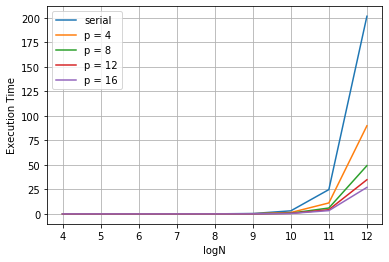
\includegraphics[width=\textwidth]{app1_exec.png}
         \caption{Approach 1 - Execution Time}
     \end{subfigure}
     \hfill
     \begin{subfigure}[b]{0.45\textwidth}
         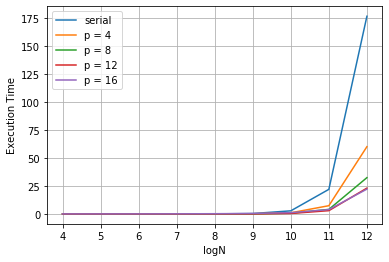
\includegraphics[width=\textwidth]{app2_exec.png}
         \caption{Approach 2 - Execution Time}
     \end{subfigure}
\end{figure}

This trend is followed by all the threads. The execution time of approach 1 is always considerably greater than the same for execution time.

% insert grph/table for serial codes only

\begin{table}[!h]
\centering
\begin{tabular}{|l|l|l|l|} \hline
Problem Size & Serial Time for approach 1 &Serial Time for approach 2 & \% Change \\ \hline

256       & 0.057               & 0.045                  & 21.05    \\
512       & 0.413               & 0.349                  & 15.50    \\
1024       & 3.137               & 2.761                  & 12.00    \\
2048      & 24.855               & 21.973                 & 11.59    \\
4096        & 201.371               & 176.583                  & 12.30    \\
\hline
\end{tabular}
\end{table}


\subsection{Speedup with Naive Parallelisation}
\begin{wrapfigure}{r}{0.7\textwidth} %this figure will be at the right
    \centering
    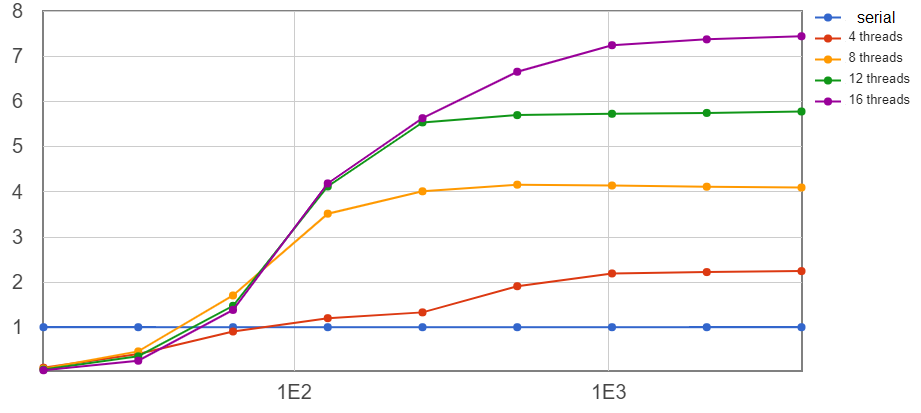
\includegraphics[width=0.7\textwidth]{app1_speedup.png}
\end{wrapfigure}
The speedup for approach 1 for 4 thread was observed as $2.224$. The reason for this is that when cores work parallely, they encounter more than $\frac{N}{16}$ misses due to possible overlap between the data fetches. Hence along with the slow execution time, we get a slower speedup as well. This remains the trend for all parallelisations i.e. using 4 threads to 8 threads. This speedup can be increased if these cache misses are avoided.
\\ \\ 

\subsection{Speedup using Auxiliary Arrays}
\begin{wrapfigure}{r}{0.7\textwidth} %this figure will be at the right
    \centering
    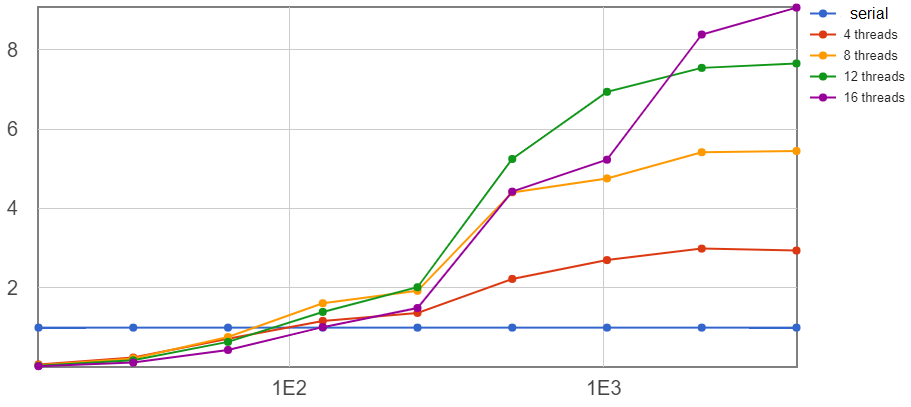
\includegraphics[width=0.7\textwidth]{app2_speedup.png}
\end{wrapfigure}

In the second approach we are using two matrix which can be \textbf{easily fit in L1 cache and thus causes lesser cache miss}. That results in a significant speedup when we consider the serial code of the same approach.

This means that serially this approach performs better than the naive serial approach and since it also suffers less cache misses, the speedup is more than the naive parallelisation as discussed previously in sections 6.2 and 6.4.


\begin{table}[!h]
\centering
\begin{tabular}{|l|l|l|l|} \hline
Thread 4/ N = 4096 & Serial Execution Time & Parallel Execution Time & Speedup \\ \hline
Approach 1         & 201.625               & 89.885                  & 2.24    \\
Approach 2         & 176.45                & 60.011                  & 2.95    \\ \hline
\end{tabular}
\end{table}

\newpage

%lolwa %shu thayu ??? 
\subsection{Efficiency}
%\begin{wrapfigure}{r}{0.5\textwidth} %this figure will be at the %right
%    \centering
%    \includegraphics[width=0.5\textwidth]{eff.jpg}
%\end{wrapfigure}


According to Amdahl's law, the theoretical speedup can not be increased more than some extent. As the serial fraction of the code is very small, according to the law, the tighter bound for speedup of our approaches is the total number of the thread used. However, parallelisation overhead and cache misses restrict the speedup to the certain amount.Note that, for smaller input size, the cache misses is not going to happen because all arrays can be fit in cache itself. But read-write overhead in approach 2 will be higher putting efficiency down for smaller inputs. Whereas for large input, the cache misses and accessing time of div[i][j] in the approach 1 causes the delay in the execution time compare to approach 2. Thus from the definition of the efficiency $$e = \frac{\mathrm{Speedup}}{\mathrm{Thread}}$$ the efficiency for approach 2 is higher than the efficiency of approach 1. 
\begin{figure}[!h]
    \centering
    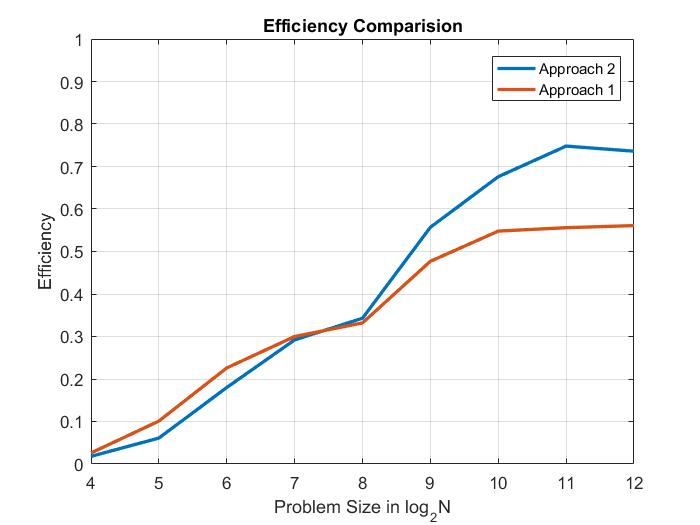
\includegraphics[scale = 0.3]{eff_4.jpg}
    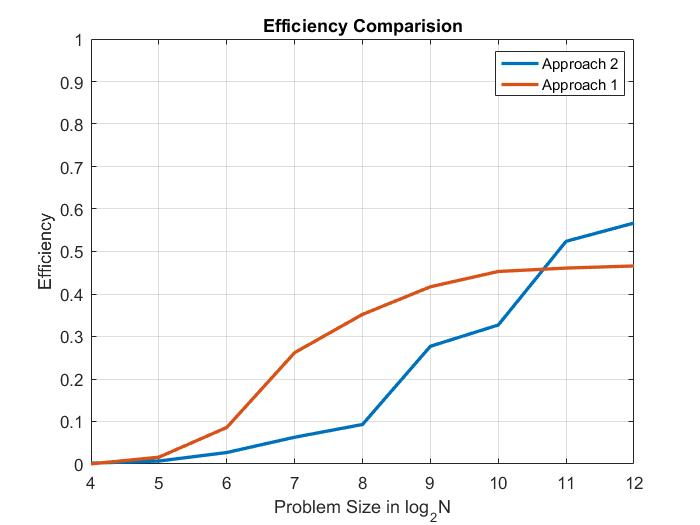
\includegraphics[scale = 0.3]{eff_16.jpg}
    \caption{Efficiency Comparison a) 4 Threads b) 16 Threads}
\end{figure}

\section{Analysis and Justifications}
\subsection{Memory Access Pattern}
\begin{figure}[!h]
    \centering
    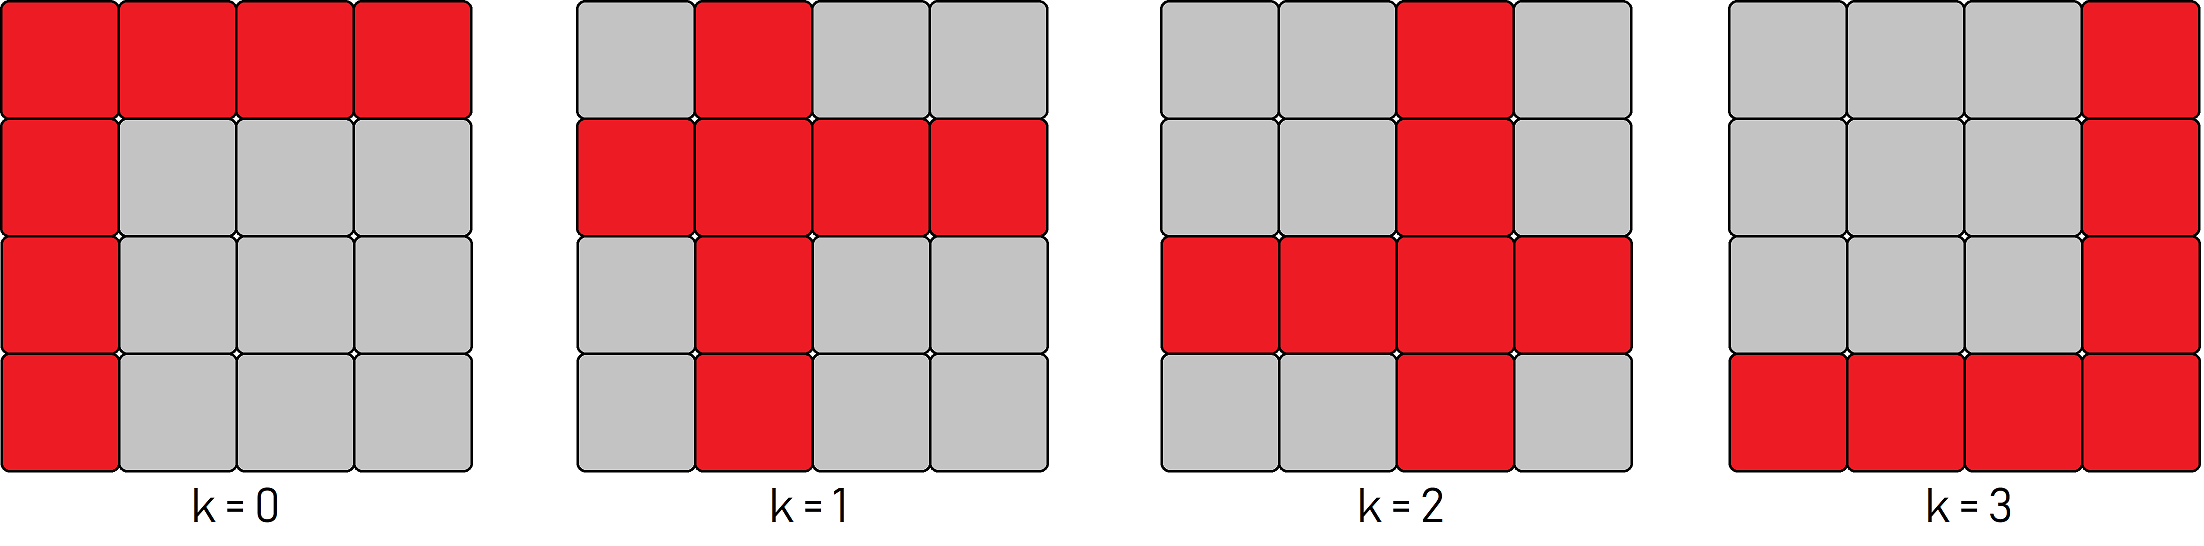
\includegraphics[scale=0.23]{memAccessPattern.png}
    \caption{Memory Access Pattern for the Algorithm}
\end{figure}

The code access the memory in the following way. An update on element $dis[i][j]$ in the $\mathrm{k}^{\mathrm{th}}$ iteration requires the $i^{th}$ value in the $\mathrm{k}^{\mathrm{th}}$ column and the $j^{th}$ value in the $\mathrm{k}^{\mathrm{th}}$ row. The two auxiliary arrays i.e. the $\mathrm{k}^{\mathrm{th}}$ row and column move in the following manner during the algorithm. 
Our main focus during parallelisation would lie on optimising the access of these arrays since the algorithm requires synchronisation between each iteration and the updates are completely parallelisable for a given iteration and can't be avoided. The cache line is of size 64 bytes. Hence each miss fetches the next 16 integers as well in the memory.
2 arrays of size $2^{12}$ can be fit into L1 cache. ($2^{12} \mathrm{elements} \times 4 \mathrm{(sizeof(int))} \times 2 \mathrm{arrays} = 32$K). Hence for a problem size $=4096$, both the column and the row can fit in the cache.

\subsection{Case 1: $2N \leq C$ and $C << N^2$}
\subsubsection{Approach 1}
\begin{enumerate}
    \item We require the entire $\mathrm{k}^{\mathrm{th}}$ row which would be available in L1 cache after one iteration of $i$ incurring $\frac{N}{16}$ misses. 
    \begin{enumerate}
        \item Serially: $\frac{N}{16}$ misses
        \item Parallely: In addition to the above misses, we will also experience misses when some processors require the same element of the $\mathrm{k}^{\mathrm{th}}$ row but both find it absent in the cache. In the worst case if the processors are working on the same index of $i$ everytime, then we can see that this will happen $p\frac{N}{16}$ times.
    \end{enumerate}
    \item We also require the entire $\mathrm{k}^{\mathrm{th}}$ column.
    \begin{enumerate}
        \item Serially: We will get $N$ misses, 1 for each row (since after the first miss, it will be there in L1 cache)
        \item Parallely: Because one row is assigned to only one core, we will get no more than $N$ misses for the column.
    \end{enumerate}
    \item We will also incur misses for accessing \texttt{dis[i][j]}. We can see that such misses are bound to occur no matter what we do.
\end{enumerate}
Thus we can conclude that the naive approach requires the same amount of cache to store the required data but also experience more misses as compared to the serial code when implemented parallely.

\subsubsection{Approach 2}
\begin{enumerate}
    \item We again need to copy the entire $\mathrm{k}^{\mathrm{th}}$ row again to the auxiliary arrays.
    \begin{enumerate}
        \item Serially: We experience the same number of cache misses as in the naive approach i.e. $\frac{N}{16}$
        \item Parallely: This time the row itself is divided amongst the processors. So each miss is unique and won't be repeated by any processor like in the naive approach.
    \end{enumerate}
    \item We need the entire $\mathrm{k}^{\mathrm{th}}$ column in this approach too. The behaviour is same as the previous approach.
    \item We will again experience misses for accessing \texttt{dis[i][j]}.
\end{enumerate}
After analysing both the parallel approaches, we can see that using auxiliary arrays, we are experiencing less misses as compared to the naive approach. Thus in the worst case the naive approach experiences $p\frac{N}{16}$ more misses and in the best case, both the approaches experience the same number of misses. However both are pathological situations and are very unlikely to happen during runtime so approach 2 performs better.

\subsection{Case 2: $C << 2N$}
In this case will experience cache misses since the $\mathrm{k}^{\mathrm{th}}$ column/row or auxiliary arrays wouldn't fit in the cache.
\subsubsection{Approach 1}
\begin{enumerate}
    \item We will now get a miss for every row when accessing \texttt{dis[k][j]} as opposed to case 1 when we used to get a miss only once for a value of $k$.
    \begin{enumerate}
        \item Serially: For one iteration of $i$, we get $\frac{N}{16}$ misses. So for the entire algorithm, we will get $\frac{N^3}{16}$ misses.
        \item Parallely: It is possible for cores to access the same memory location resulting in $p\frac{N^3}{16}$ misses in the worst case.
    \end{enumerate}
    \item While accessing the $\mathrm{k}^{\mathrm{th}}$ column we have:
    \begin{enumerate}
        \item Serially: While accessing \texttt{dis[i][k]}, we get 1 miss per row. So there would be $N^2$ misses.
        \item Parallely: Again all the misses are unique like in case 1 i.e. we get $N^2$ misses.
    \end{enumerate}
    \item Accessing \texttt{dis[i][j]} results in a total of $\frac{N^3}{16}$ misses.
\end{enumerate}

\subsubsection{Approach 2}
\begin{enumerate}
    \item While loading the auxiliary arrays, it is clear that we will experience $\frac{N}{16} + N$ misses for each $k$ or $\frac{N^2}{16} + N^2$ for the entire algorithm.
    \item The analysis done for accessing the $\mathrm{k}^{\mathrm{th}}$ row is duplicated but this time for the auxiliary array
    \item We will now experience lower cache misses when accessing \texttt{dis[i][k]} because now it is replaced by a contiguous auxiliary array.
    \begin{enumerate}
        \item Serially: Reduced to $\frac{N^2}{16}$
        \item Parallely: Reduced to $\frac{N^2}{16}$
    \end{enumerate}
    \item Accessing \texttt{dis[i][j]} results in a total of $\frac{N^3}{16}$ misses.
\end{enumerate}
Concluding we have,
\begin{itemize}
    \item Naive Parallel: $p\frac{N^3}{16} + N^2 + \frac{N^3}{16}$ misses
    \item Approach 2: $\frac{N^2}{16} + N^2 + p\frac{N^3}{16} + \frac{N^2}{16} + \frac{N^3}{16}$ misses
\end{itemize}
Analysing both the parallel approaches we see that, approach 2 has an extra $\frac{N^2}{8}$ misses. However approach 2 has a compute advantage over the naive approach which is explained in the next section.

\subsection{Compute Costs}
The memory allocated for the \texttt{dis} array is linear so when we access \texttt{dis[i][j]}, the offset calculation takes about 10 cycles for multiplication since we need to calculate offset $=i \times N + j$. There are 2 such operations (\texttt{dis[i][k]} and \texttt{dis[k][j]}) in each update which mean $2N^3$ such operations.

There are 2 possible ways to remove this computation.
\begin{enumerate}
    \item Store the values contiguously as we did in approach 2. Here we see that the code remains parallelisable but we incur an extra $\frac{N^2}{8}$ cache misses.
    \item Use a contiguous array but calculate the offset at each iteration by adding $k$ to the previous offset with initial offset being equal to $i$. This adds an extra computation of 1 cycle but that is still better than 1 multiplication instance. However note that this introduces a dependency in the algorithm and hence can't be parallelised anymore. 
\end{enumerate}
In addition to the above observations, let us see when compute costs advantage overcome the memory access disadvantage. Assuming that a L3 cache miss means a penalty of 1000 cycles and a multiplication operation takes 5 cycles, we find that the turning point of $N$ is,

$$(2N^3) \times 5 > (\frac{N^2}{8}) \times 1000$$
$$N > \lceil \frac{100}{8} \rceil \implies N > 13$$

Thus we conclude that the time saved in compute costs of offsets have overcome the cache miss penalties far earlier and even in those cases approach 2 remains the better one since the cache contains the auxiliary array before the core algorithm begins.

\subsection{Scheduling Policies}
In the schedule(static, chunk-size) scheduling policy, OpenMP divides the iterations into chunks of size chunk-size and it distributes the chunks to threads in a circular order. In the schedule(dynamic, chunk-size) scheduling type, OpenMP divides the iterations into chunks of size chunk-size. Each thread executes a chunk of iterations and then requests another chunk until there are no more chunks available. Here two terms are important to understand.
\begin{itemize}
    \item \textbf{Scheduling Overhead:} Since dynamic scheduling divide the work load among thread according to their availability, every time a thread is idle it has to be assigned to a chunk by the OS. This scheduling will cause a delay in the run time called as "Scheduling Overhead".
    \item \textbf{Load Balance:} Load balance means "Equal work to all threads". Dynamic scheduling automatically assigns the work to that thread which is available causing no delay in the run time. Whereas static scheduling algorithm assign the work depending upon the chunk size.
\end{itemize}
Since we observed that there are no condition checks inside the parallel region and all thread have to do a fix amount of work on each iteration. Thus the work load can be evenly distributed among threads at compile time and we can get rid of dynamic scheduling overhead.
\begin{table}[!h]
\centering
\begin{tabular}{|l|l|l|l|} \hline
Thread 4/ N = 4096 & Serial Execution Time & Parallel Execution Time & Speedup \\ \hline
Dynamic         & 189.479                &     74.609              &     2.54 \\
Static         & 176.45                & 60.011                  & 2.95    \\ \hline
\end{tabular}
\end{table}


\section{Conclusion}
After all analysis we can say that using auxiliary arrays results in an improvement in the serial algorithm by reducing computation incurred in offset calculation while maintaining the same if not less cache miss rate. Removing these computation costs in the naive approach requires introduction of dependencies which renders the algorithm unparallelisable. Using auxiliary arrays has it's own compute costs and overheads but doing so allows us to parallelise the problem and still get a considerable improvement over the naive approach.

\section{References}
\begin{itemize}
    \item Basics of the serial Floyd-Warshall Algorithm:
    \begin{itemize}
        \item \url{https://en.wikipedia.org/wiki/Floyd\%E2\%80\%93Warshall\_algorithm}
    \end{itemize}
    \item Contiguous Memory Allocation Syntax:
    \begin{itemize}
        \item \url{https://stackoverflow.com/questions/13105056/allocate-contiguous-memory}
    \end{itemize}
    \item Scheduling Policies:
    \begin{itemize}
        \item \url{http://jakascorner.com/blog/2016/06/omp-for-scheduling.html} 
        \item \url{https://people.sc.fsu.edu/~jburkardt/c\_src/schedule\_openmp/schedule\_openmp.html}
    \end{itemize}
    
    
\end{itemize}

\newpage
\section{Appendix}
\subsection*{Compute Node Specs}
\begin{table}[!h]
\centering
\begin{tabular}{|l|l|}
\hline
Architecture & x86\_64 \\
Cores & 16 \\
Threads per Core & 1 \\
Sockets  & 2 \\
CPUs per Socket  & 8 \\ 
Model & Intel Xeon E5-2640 v3 @ 2.60GHz \\
L1 Cache & 32K  \\
L2 Cache & 256K\\
L3 Cache & 20480K\\ \hline
\end{tabular}
\end{table}

\subsection*{Naive Parallelisation Static Scheduling}
\begin{table}[!h]
\centering
\begin{tabular}{|c|c|c|c|c|c|} \hline
$N$ & serial & $p=4$ & $p=8$ & $p=12$ & $p=16$\\ \hline
64 & 0.001 & 0.001 & 0.001 & 0.001 & 0.001\\
128 & 0.008 & 0.007 & 0.002 & 0.002 & 0.002\\
256 & 0.056 & 0.043 & 0.014 & 0.010 & 0.010\\
512 & 0.411 & 0.216 & 0.099 & 0.072 & 0.062\\
1024 & 3.129 & 1.429 & 0.755 & 0.546 & 0.042\\
2048 & 24.824 & 11.184 & 6.033 & 4.317 & 3.363\\
4096 & 201.625 & 89.885 & 49.228 & 34.867 & 27.059\\ \hline
\end{tabular}
\end{table}

\subsection*{Using Auxiliary Arrays and Static Scheduling}
\begin{table}[!h]
\centering
\begin{tabular}{|c|c|c|c|c|c|} \hline
$N$ & serial & $p=4$ & $p=8$ & $p=12$ & $p=16$\\ \hline
64 & 0.001 & 0.001 & 0.001 & 0.001 & 0.039\\
128 & 0.006 & 0.005 & 0.004 & 0.004 & 0.086\\
256 & 0.044 & 0.033 & 0.023 & 0.022 & 0.186\\
512 & 0.348 & 0.157 & 0.079 & 0.066 & 0.394\\
1024 & 2.754 & 1.019 & 0.579 & 0.397 & 1.122\\
2048 & 21.937 & 7.336 & 4.047 & 2.907 & 3.855\\
4096 & 176.45 & 60.011 & 32.376 & 23.039 & 22.194\\ \hline
\end{tabular}
\end{table}

\subsection*{Using Auxiliary Arrays and Dynamic Scheduling}
\begin{table}[!h]
\centering
\begin{tabular}{|c|c|c|c|c|c|} \hline
$N$ & serial & $p=4$ & $p=8$ & $p=12$ & $p=16$\\ \hline
64   & 0.001 & 0.002 & 0.002 & 0.002 &  0.002 \\
128  & 0.007 & 0.008 & 0.006 & 0.007 &  0.007 \\
256  & 0.051 & 0.039 & 0.025 & 0.025 &  0.027 \\ 
512  & 0.372 & 0.186 & 0.119 & 0.101 &  0.093 \\
1024 & 2.951 & 1.243 & 0.761 & 0.601 &  0.525 \\
2048 & 23.565 & 9.339 & 5.393 & 4.017 & 3.297 \\
4096 & 189.479 & 74.604 & 41.358 & 30.096 & 23.888 \\ \hline
\end{tabular}
\end{table}



\end{document}